\subsection{Analisi delle ridondanze}
\subsubsection{Attributo COSTO TOTALE}
All'interno dello schema ER è stata identificato l'attributo \textbf{costo totale}, nella Entità "Prenotazione" come ridonante.\\\\
L'attributo ci permette di gestire il costo totale della prenotazione senza dover calcolarlo a partire dall'attributo \textbf{costo} di "Alloggio" (inteso come costo per notte), sommandolo al \textbf{costo pulizia}.

\small
\setlength\extrarowheight{2pt}
\begin{longtable}{|c|p{3cm}|c|c|p{4.18cm}|}
      \hline \# & \textbf{Concetto}           & \textbf{Tipo} & \textbf{Volume} & \textbf{Motivazione}                                          \\\hline
      \endfirsthead

      \hline \# & \textbf{Concetto}           & \textbf{Tipo} & \textbf{Volume} & \textbf{Motivazione}                                          \\\hline
      \endhead

      \endfoot

      \endlastfoot
      2         & Prenotazione di un alloggio & {I}           & 25.000/day      & Operazione principale che permette di effettuare un soggiorno \\\hline
\end{longtable}
\normalsize

\begin{figure}[H]
      \centering
      \begin{minipage}[b]{0.3\textwidth}
            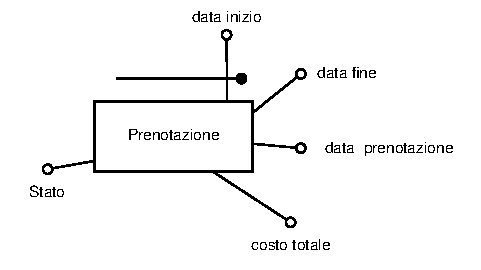
\includegraphics[width=\textwidth]{resources/pdf/page5.pdf}
            \caption{Con ridondanza}
      \end{minipage}
      \centering
      \begin{minipage}[b]{0.6\textwidth}
            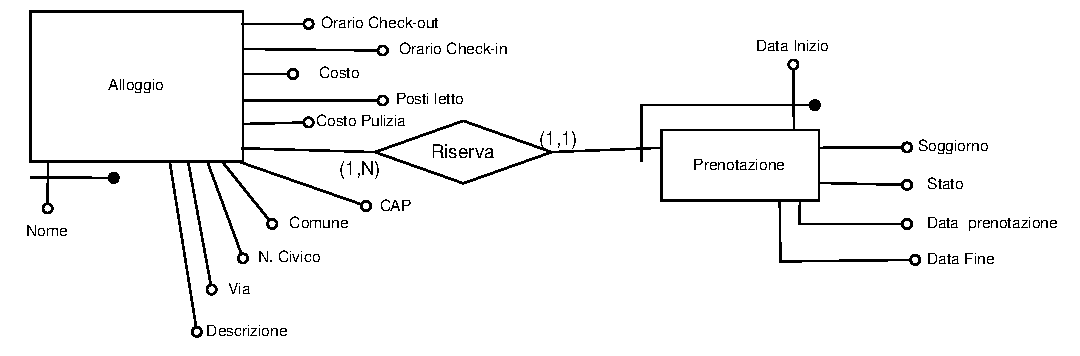
\includegraphics[width=\textwidth]{resources/pdf/page6.pdf}
            \caption{Senza ridondanza}
      \end{minipage}
\end{figure}

\clearpage
\subsubsection{Tavola degli accessi}
Analizziamo l'operazione "\textbf{Prenotazione di un alloggio (25.000 volte al giorno)}"

\small
\setlength\extrarowheight{2pt}
\begin{longtable}{|lccc|}
      \caption*{In presenza di ridondanza}                                             \\

      \hline \textbf{Concetto} & \textbf{Costrutto} & \textbf{Accessi} & \textbf{Tipo} \\\hline
      \endfirsthead

      \hline \textbf{Concetto} & \textbf{Costrutto} & \textbf{Accessi} & \textbf{Tipo} \\\hline
      \endhead

      \hline \multicolumn{4}{|r|}{{Continua all pagina successiva}}                    \\\hline
      \endfoot

      \hline
      \endlastfoot
      Prenotazione             & E                  & 1                & L             \\%\hline
      Prenotazione             & E                  & 1                & S             \\%\hline
\end{longtable}
\normalsize

\small
\setlength\extrarowheight{2pt}
\begin{longtable}{|lccc|}
      \caption*{Senza la ridondanza}   \\

      \hline \textbf{Concetto} & \textbf{Costrutto} & \textbf{Accessi} & \textbf{Tipo} \\\hline
      \endfirsthead

      \hline \textbf{Concetto} & \textbf{Costrutto} & \textbf{Accessi} & \textbf{Tipo} \\\hline
      \endhead

      \hline \multicolumn{4}{|r|}{{Continua all pagina successiva}}                    \\\hline
      \endfoot

      \hline
      \endlastfoot
      Prenotazione             & E                  & 1                & S             \\%\hline
      Prenotazione             & E                  & 1                & L             \\%\hline
      Riserva                  & R                  & 1                & L             \\%\hline
      Alloggio                 & R                  & 1                & L             \\%\hline
\end{longtable}
\normalsize


% 
% 
%      TUTTE LE IMMAGINI DI QUESTA PAGINA VANNO MESSE A COPPIE, 2 IMMAGINI PER PAGINA UNA ACCANTO ALL'ALTRA
% 
%

Analisi di complessità \myuline{in presenza di ridondanza}:
\begin{itemize}
      \item In termini di tempo
      \begin{itemize}
            \item vengono effettuati un accesso in lettura ed uno in scrittura, per un totale di 75.000 accessi (contiamo doppi gli accessi in scrittura)
      \end{itemize}
      \item In termini di spazio
      \begin{itemize}
            \item Il costo totale viene memorizzato come un intero a 4 byte, ipotizzando 36.000.000 di prenotazioni, lo spazio totale necessario è di $\thickapprox 144$ Mb.
      \end{itemize}
\end{itemize}

Analisi di complessità \myuline{in assenza di ridondanza}:
\begin{itemize}
      \item In termini di spazio
      \begin{itemize}
            \item il costo totale è 0 byte.
      \end{itemize}
      \item In termini di tempo
      \begin{itemize}
            \item vengono effettuati tre accessi in lettura e un accesso in scrittura, per un totale di 125.000 accessi.
      \end{itemize}
\end{itemize}
Dall'analisi effettuata, con l'assenza di ridondanza, risulta un peggioramento nei tempi di accesso (circa il 67\% di tempo in più) ed un risparmio discreto in termini di spreco di memoria; essendo l'operazione usata con molta frequenza ed in maniera interattiva \myuline{preferiamo mantenere la ridondanza}.

\subsection{Eliminazione delle generalizzazioni}
\subsubsection{Entità RECENSIONE}
\begin{figure}[H]
      \centering
      \begin{minipage}[b]{0.45\textwidth}
            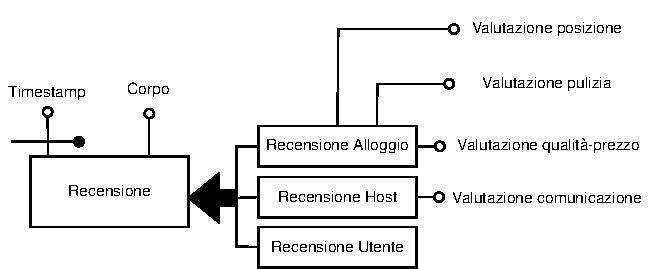
\includegraphics[width=\textwidth]{resources/pdf/page7.pdf}
            \caption{Prima}
      \end{minipage}
      \hfill
      \begin{minipage}[b]{0.45\textwidth}
            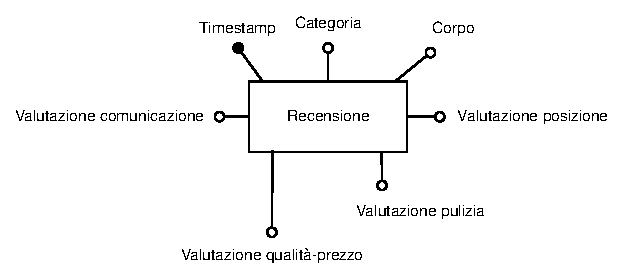
\includegraphics[width=\textwidth]{resources/pdf/page8.pdf}
            \caption{Dopo}
      \end{minipage}
      \caption*{La generalizzazione è di tipo \textbf{totale ed esclusiva}. La decisione consiste nel raggruppamento delle entità	figlie nell'attributo categoria. Gli attributi specifici delle entità figlie (valutazioni) vengono spostate nell'entità padre, diventando annullabili. L'attributo categoria sarà un valore not null.}
\end{figure}

\subsubsection{Entità ALLOGGIO}
\begin{figure}[H]
      \centering
      \begin{minipage}[b]{0.45\textwidth}
            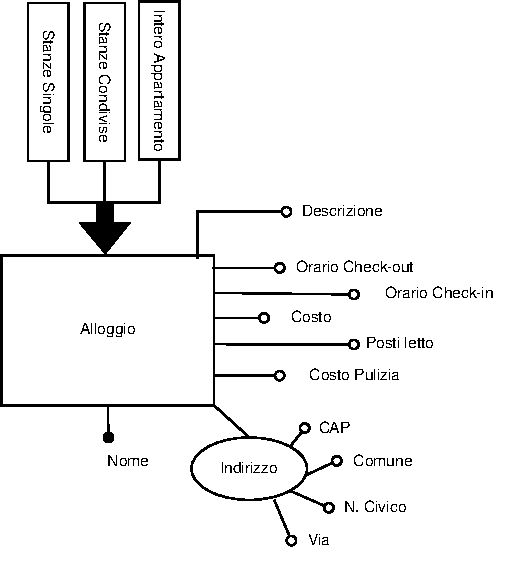
\includegraphics[width=\textwidth]{resources/pdf/page9.pdf}
            \caption{Prima}
      \end{minipage}
      \hfill
      \begin{minipage}[b]{0.45\textwidth}
            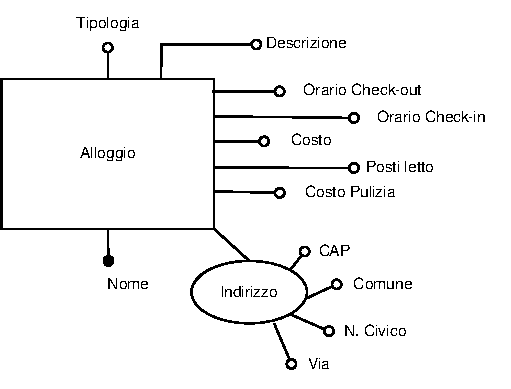
\includegraphics[width=\textwidth]{resources/pdf/page10.pdf}
            \caption{Dopo}
      \end{minipage}
      \caption*{La generalizzazione è di tipo \textbf{totale ed esclusiva}. La decisione consiste nel raggruppamento delle entità	figlie nell'attributo tipologia, con valore not null.}
\end{figure}

\subsubsection{Entità UTENTE}
\begin{figure}[H]
      \centering
      \begin{minipage}[b]{0.45\textwidth}
            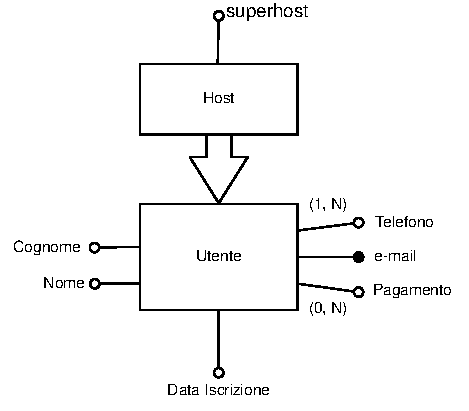
\includegraphics[width=\textwidth]{resources/pdf/page11.pdf}
            \caption{Prima}
      \end{minipage}
      \hfill
      \begin{minipage}[b]{0.45\textwidth}
            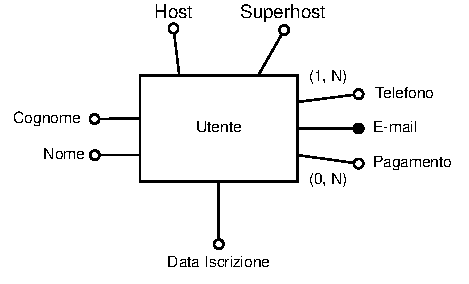
\includegraphics[width=\textwidth]{resources/pdf/page12.pdf}
            \caption{Dopo}
      \end{minipage}
      \caption*{La generalizzazione è di tipo \textbf{parziale e sovrapposta}. La decisione consiste nel raggruppamento dell'entità figlia nell'attributo host, con valore not null. L'attributo superhost dell'entità figlia viene trasferito al padre.}
\end{figure}


\subsection{Partizionamento/accorpamento di entità e associazioni}
\subsubsection{Accorpamento Entità PRENOTAZIONE e SOGGIORNO}
\begin{figure}[H]
      \centering
      \begin{minipage}[b]{0.45\textwidth}
            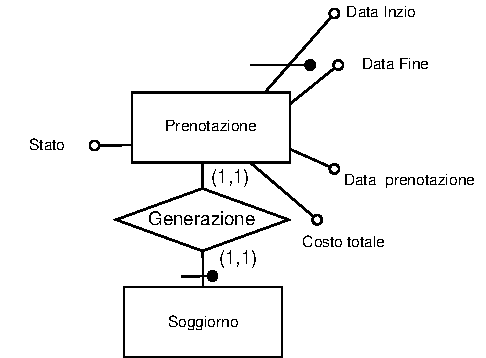
\includegraphics[width=\textwidth]{resources/pdf/page13.pdf}
            \caption{Prima}
      \end{minipage}
      \hfill
      \begin{minipage}[b]{0.45\textwidth}
            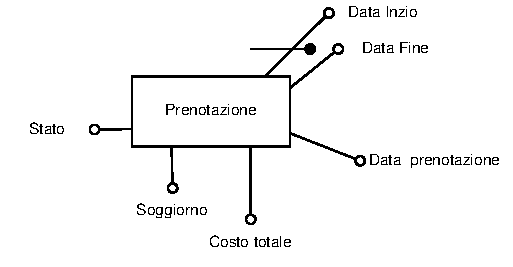
\includegraphics[width=\textwidth]{resources/pdf/page14.pdf}
            \caption{Dopo}
      \end{minipage}
      \caption*{La decisione di accorpare le entità Prenotazione e Soggiorno in un'unica entità con attributo soggiorno (di tipo booleano) deriva dal fatto che l'entità Soggiorno viene generata dalle prenotazioni con stato "confermata".}
\end{figure}

\subsubsection{Partizionamento Entità UTENTE}
\begin{figure}[H]
      \centering
      \begin{minipage}[b]{0.27\textwidth}
            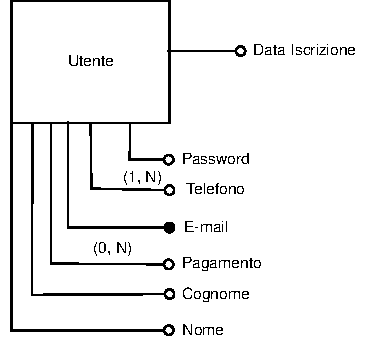
\includegraphics[width=\textwidth]{resources/pdf/page15.pdf}
            \caption{Prima}
      \end{minipage}
      \hfill
      \begin{minipage}[b]{0.63\textwidth}
            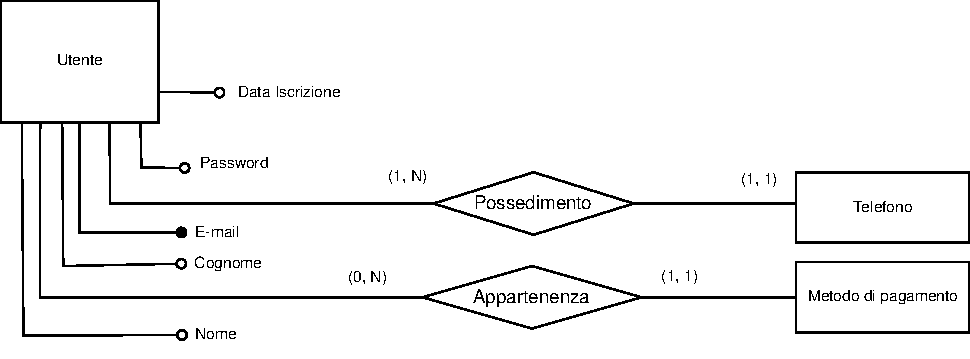
\includegraphics[width=\textwidth]{resources/pdf/page16.pdf}
            \caption{Dopo}
      \end{minipage}
      \caption*{Decidiamo di partizionare l'entità Utente estraendo gli attributi telefono e pagamento, facendoli diventare rispettivamente una nuova entità Telefono, associata a Utente tramite la relazione Possedimento, e una nuova entità Pagamento, associata a Utente tramite la relazione Appartenenza.}
\end{figure}

\subsubsection{Partizionamento Entità ALLOGGIO}
\begin{figure}[H]
      \centering
      \begin{minipage}[b]{0.40\textwidth}
            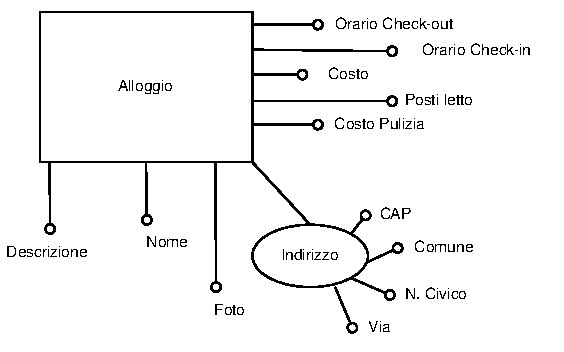
\includegraphics[width=\textwidth]{resources/pdf/page17.pdf}
            \caption{Prima}
      \end{minipage}
      \hfill
      \begin{minipage}[b]{0.50\textwidth}
            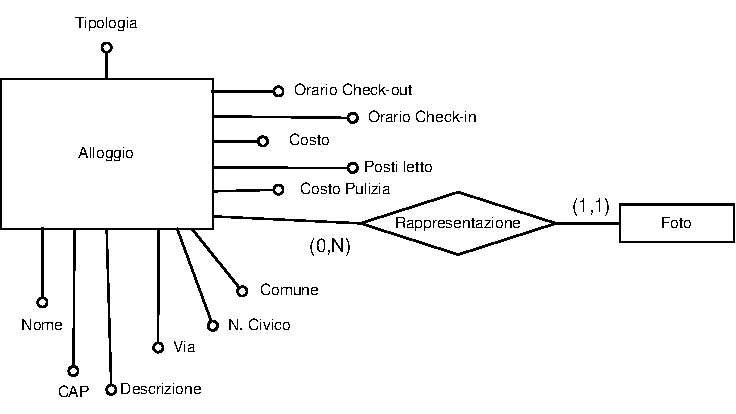
\includegraphics[width=\textwidth]{resources/pdf/page18.pdf}
            \caption{Dopo}
      \end{minipage}
      \caption*{Decidiamo di partizionare l'entità Alloggio estraendo l'attributo foto, facendolo diventare una nuova entità Foto, associata a Alloggio tramite la relazione Rappresentazione.}
\end{figure}

\subsection{Eliminazione degli attributi composti}
L’attributo composto “\textbf{indirizzo}” viene eliminato, considerando i suoi componenti come attributi semplici. Nel caso di indirizzo abbiamo: via, numero civico, cap e comune.
Vedi figura 2.14.